% En-têtes LaTex
\documentclass[a4paper, 10pt]{article}

%% use for debbug layers 
%\usepackage{showframe}

\usepackage{lmodern}
\usepackage{moreverb}
\usepackage{multicol}
\usepackage[a4paper,left=2cm,right=2cm,top=2cm,bottom=2cm]{geometry}
\usepackage{array}
\usepackage{enumitem}
\usepackage{arydshln}  % Pour les lignes en pointillés
\usepackage[table]{xcolor}  % Pour la coloration des cellules
\usepackage{amsmath}  % For the \text command


% ***************************************%
%               typography               %
% ***************************************%
\usepackage[french]{babel} % Règles typographiques françaises
\usepackage[T1]{fontenc}
\usepackage[utf8]{inputenc} % Pour les caractères accentués

\usepackage{tgbonum}
\usepackage{enumitem}
\setlist[itemize]{label=$\bullet$}
%%% Create new type of list %%%
\newlist{gitemize}{itemize}{4}
\setlist[gitemize,1]{
  leftmargin=\dimexpr0.3cm+\labelsep\relax,
  label={\smash{\raisebox{-0.25\height}{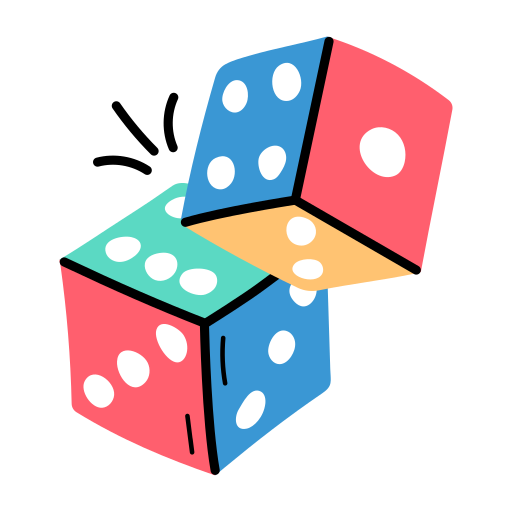
\includegraphics[width=0.35cm]{img/bullet/dice.png}}}}
}


% ***************************************%
%                 links                  %
% ***************************************%
\usepackage{hyperref}
\hypersetup{
    colorlinks=true,
    breaklinks=true, %permet le retour à la ligne dans les liens trop longs
    linkcolor=blue,
    filecolor=magenta,      
    urlcolor=cyan,
    pdftitle={Intéropérabilité-AlpesTransport},
    pdfpagemode=FullScreen,
    }
\urlstyle{same}



% ***************************************%
%       Including graphics documents     %
% ***************************************%
\usepackage{graphicx} % To insert graphics
\usepackage{float} % To allow floating images around text
\usepackage{wrapfig} % to make float figures
\usepackage{psfrag} % to modify text of a figure.



\pagestyle{headings}
\pagestyle{plain}


\makeatletter

\makeatother

\makeatletter
\def\toclevel@subsubsubsection{4}
\def\toclevel@paragraph{5}
\def\toclevel@subparagraph{6}
\makeatother


%\setlength{\parindent}{0cm}
\setlength{\parskip}{1ex plus 0.5ex minus 0.2ex}

% ***************************************%
%            style of titles             %
% ***************************************%
\setcounter{secnumdepth}{5} % pour numéroter les sections jusqu'au subparagraph
\setcounter{tocdepth}{5}
\usepackage{titlesec}
\usepackage{titletoc}% pour modifier la couleur dans le table of content
\usepackage{xcolor}
\usepackage{tocloft}  

% Définir les couleurs des sections
\colorlet{sectioncolor}{purple}
\colorlet{subsectioncolor}{teal}
\colorlet{subsubsectioncolor}{olive}

% Définir les commandes \titleformat pour les sections
\titleformat{\section}
	{\color{sectioncolor}\normalfont\Large\bfseries}
	{\color{sectioncolor}\thesection}{2em}{}

\titleformat{\subsection}
	{\color{subsectioncolor}\normalfont\Large\bfseries}
	{\color{subsectioncolor}\thesubsection}{1em}{}

\titleformat{\subsubsection}
	{\color{subsubsectioncolor}\normalfont\bfseries}
	{\color{subsubsectioncolor}\thesubsubsection}{1em}{}

% Redéfinir la commande \cftsecfont pour utiliser la même couleur que les sections
\renewcommand{\cftsecfont}{\color{sectioncolor}\normalfont}
\renewcommand{\cftsubsecfont}{\color{subsectioncolor}\normalfont}
\renewcommand{\cftsubsubsecfont}{\color{subsubsectioncolor}\normalfont}

% Modifier la couleur des numéros de section dans la table des matières
\titlecontents{section}
    [0em]
    {\color{sectioncolor}}
    {\contentslabel{2em}}
    {\hspace*{2em}}
    {\titlerule*[0.5pc]{.}\contentspage}

\titlecontents{subsection}
    [2em]
    {\color{subsectioncolor}}
    {\contentslabel{2.5em}}
    {\hspace*{2.5em}}
    {\titlerule*[0.5pc]{.}\contentspage}

\titlecontents{subsubsection}
    [4.5em]
    {\color{subsubsectioncolor}}
    {\contentslabel{3em}}
    {\hspace*{3em}}
    {\titlerule*[0.5pc]{.}\contentspage}



% ***************************************%
%          Personilized commands         %
% ***************************************%
\newcommand{\hsp}{\hspace{20pt}}
\newcommand{\HRule}{\rule{\linewidth}{0.5mm}}

%% specific color for this report chosen like the powerpoint ones
\definecolor{mygreen}{RGB}{6, 200, 146}
\definecolor{myblue}{RGB}{83, 131, 255}

% for displaying acronymes
\newcommand{\otp}{\textsc{OTP} }
\newcommand{\totp}{\textsc{TOTP} }
\newcommand{\hotp}{\textsc{HOTP} }
\newcommand{\hmac}{\textsc{hmac} }



% -----------------
% Début du document 
% -----------------
\begin{document}

\begin{titlepage}
  \begin{sffamily}
  \begin{center}

    \textsc{\LARGE }\\[2cm]

    \textsc{\Large Securité }\\[1.2cm]

    \HRule \\[0.4cm]
    { \huge  \textsc{One Time Password} \\ 
    [0.5cm]
    }
    \HRule \\[1cm]
        \textsc{Groupe Mohammed \textbf{ROUABAH}, William \textbf{MAILLARD}}

    \begin{figure}
        \centering
        
\includegraphics[scale=0.2]{img/ujmlogo.png}
        \label{fig:ujm_logo}
    \end{figure}

    \
\vfill
    \begin{figure}[H]
        \centering
        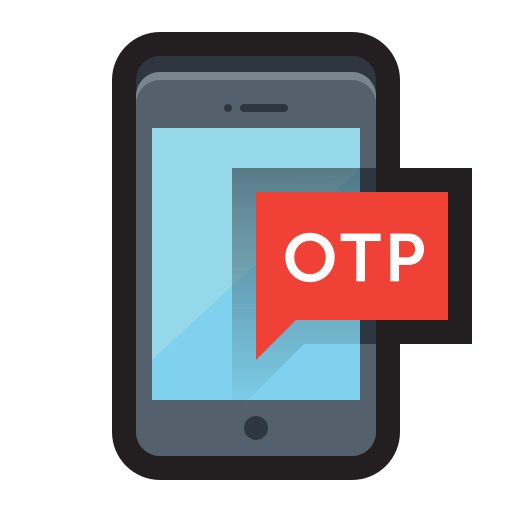
\includegraphics[scale=0.35]{img/pin.png}
        \label{fig:ujm_logo}
    \end{figure}
\vfill

    {\large {} 25/01/2023}

  \end{center}
  \end{sffamily}
\end{titlepage}



\newpage

\tableofcontents
\newpage

% ***************************************%
%  Résumé du rapport                     %
% ***************************************%
\begin{abstract}
\addcontentsline{toc}{section}{Abstract}
Ce rapport introduit les différents concepts inhérents à \textcolor{mygreen}{l'algorithme \otp} en prenant l'exemple de son utilisation dans le \textcolor{myblue}{protocole 2FA}. Ensuite il explique en détaille et en déroulant un exemple concret, les différentes partie de l'algorithme permettant de générer un \otp à partir d'une \textcolor{mygreen}{clé privé} partagé et d'une \textcolor{mygreen}{donnée incrémentale}. Puis il montre la mise en place du 2FA avec les deux \textcolor{myblue}{variantes} d'\otp, \textcolor{myblue}{\hotp} et \textcolor{myblue}{\totp}, sur un prototype réalisé en \textcolor{myblue}{python}. Finalement, ce rapport conclus en mettant en exergue les \textcolor{myblue}{failles de sécurités} possible à l'utilisation d'\otp et quelles sont les bonnes pratiques à mettre en place pour s'en prémunir.
\end{abstract}
\newpage


    \section*{Introduction}
    \addcontentsline{toc}{section}{Introduction}


%% définitions et introduction

    Un \textcolor{myblue}{mot de passe à usage unique}, désigné sous l'acronyme anglais \textcolor{myblue}{\otp} dans la suite de ce rapport, 
est une séquence d'au moins \textcolor{mygreen}{six chiffres} ou caractère généré à partir d'une \textcolor{mygreen}{clé privé} et d'une \textcolor{mygreen}{donnée itérative}
afin de \textcolor{myblue}{valider une action} utilisateur comme par exemple une authentification ou une transaction bancaire. 

    Ces codes sont soit généré avec une \textcolor{myblue}{application} dite 'authenticator' soit \textcolor{myblue}{envoyé} à l'utilisateur cherchant
à valider une action par courriel ou message. Ces codes sont donc générés par un moyen que \textcolor{mygreen}{seul l'utilisateur concerné possède}.\\


    Les \otp  sont donc tout naturellement utilisés dans les méthodes d'authentification dites '\textcolor{myblue}{2FA}'  qui consiste à vérifier que
l'utilisateur \textcolor{myblue}{possède quelque chose} en plus de connaître son mot de passe.
Plus particulièrement cela permet d'attester que l'utilisateur possède \textcolor{mygreen}{un appareil physique} (téléphone mobile ou clé otp) ou \textcolor{mygreen}{un compte virtuel} (mail ou numéro de téléphone).\\



%% exemples d'utilisation 

    D'autre part, l'utilisation des \otp ne se limitent pas au \textsc{2FA}, mais est aussi \textcolor{myblue}{utilisé dans de nombreux domaines} comme par exemple :\\
\begin{description}
    \item[Systèmes de Port Knocking :] 
    Ils utilisent des \otp pour ajouter une couche de sécurité à l'accès réseau. L'utilisateur génère un \otp valide en tapant une séquence spécifique de requêtes vers des ports prédéfinis, permettant ainsi l'ouverture temporaire de ports et l'accès au réseau.\\

    \item[Preuve de Localisation Préservant la Vie Privée :]
    Dans ce contexte, les \otp peuvent être utilisés pour valider la présence d'un individu à un endroit particulier sans révéler de données sensibles. L'individu génère un \otp qui atteste de sa localisation actuelle sans divulguer d'informations précises.\\

    \item[VPN d’Entreprise :] 
Des clés \otp permettant de générer des \totp sont utilisés dans les VPN d'entreprise pour renforcer l'authentification. Les employés utilisent ces codes pour générer des codes valides, nécessaires pour établir une connexion sécurisée au réseau de l'entreprise.\\

    \item[Validations Bancaires et de Paiement Électronique :] 
Les \otp sont couramment utilisés dans les validations bancaires et les transactions de paiement électronique. Lorsqu'un utilisateur effectue une transaction, un \otp est généré et envoyé à son appareil mobile, assurant une couche supplémentaire de sécurité en vérifiant l'authenticité de la transaction.\\
\end{description}


%% annonce du plan

    Ainsi, nous allons étudier, dans ce rapport, les \textcolor{myblue}{mécanismes cryptographiques} permettant de générer ces codes à usage unique.

    Pour cela nous analyserons l'\textcolor{myblue}{utilisation des \otp dans le protocole 2FA} afin d'en extraire des \textcolor{mygreen}{concepts }inhérents et comprendre la divergence entre les \textcolor{mygreen}{deux variante} que constituent l'\hotp et le \totp .

    Ensuite, à l'aide des concepts définis précédemment, nous construirons un \textcolor{myblue}{algorithme de génération d'\otp} , en veillant à comprendre les \textcolor{mygreen}{enjeux de sécurité} derrière chaque \textcolor{mygreen}{choix de paramètre} de cet algorithme.

    Puis nous expliquerons comment \textcolor{myblue}{intégrer une validation \otp} dans son application en s'appuyant sur le \textcolor{mygreen}{prototype python} qui a été développé dans le cadre de cette étude.

    Finalement, nous expliquerons les \textcolor{myblue}{failles de sécurité} que peut présenter l'utilisation d'\otp afin de terminer sur les \textcolor{mygreen}{points de sécurités conseillés} afin d'assurer une utilisation sécurisé de cette technologie.\\



\newpage
% ***************************************%
%  1. Exemple d'utilisation d' OTP       %
% ***************************************%
    \section{Exemple d'utilisation d'\otp dans le 2FA}


    Comme expliqué dans l'introduction les \otp sont utilisé dans le \textcolor{myblue}{protocole de double authentification} 2FA visant à vérifier que \textcolor{mygreen}{l'utilisateur possède quelque chose} en plus de vérifier la connaissance de son mot de passe.\\

    Dans cette partie nous allons ainsi nous intéressé aux \textcolor{myblue}{application 'authenticator'} permettant de générer des \otp en étudiant dans un premier temps quels sont les \textcolor{mygreen}{mécanismes} à mettre en place \textcolor{mygreen}{pour activer le 2FA}. 
    
    Puis, dans un second temps, nous verrons comment l'\otp permet de \textcolor{myblue}{valider l'authentification} de l'utilisateur dans le contexte du 2FA, et \textcolor{myblue}{les variantes} que constituent \textcolor{mygreen}{\hotp} et \textcolor{mygreen}{\totp} . 
    
    Et enfin nous déduirons de ces exemples les paramètres à prendre en compte pour palier les \textcolor{myblue}{désynchronisation de génération d'\otp} entre le client et le serveur.


        %% ***** Partage de seed ***** %%
        \subsection{Activation du 2FA : partage de secret entre le client et le serveur}

    Afin d'attester de l'identité d'un client avec un code \otp\ , il faut que chaque partie (le client et le serveur) possède \textcolor{myblue}{un moyen de générer des codes identiques}. 
Ainsi lorsque l'utilisateur active le 2FA sur son compte le serveur va créer et \textcolor{mygreen}{communiquer une clé secrète} au client avant de lui même \textcolor{myblue}{stocker} cette valeur.
Cette clé va servir de \textcolor{myblue}{graine}, ou seed en anglais, à la \textcolor{myblue}{génération d'\otp\ identiques} du côté du client et du serveur permettant à ce dernier d'attester l'identité du premier.\\

    Le \textcolor{myblue}{partage} de cette clé secrète est réalisé à travers la génération d'un \textcolor{mygreen}{QRcode} par le serveur et le scanne de ce dernier par le client utilisant une application 'authenticator' comme freeOTP. L'exemple ci-dessous montre le contenus d'un exemple de QRcode généré pour activer le 2FA d'un compte github.\\


\begin{figure}[H]
        \centering
        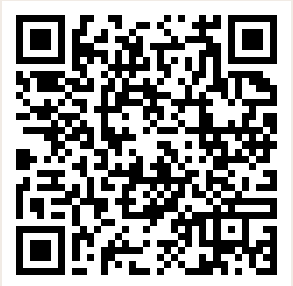
\includegraphics[scale=0.5]{img/1/1/qrcode.png}
        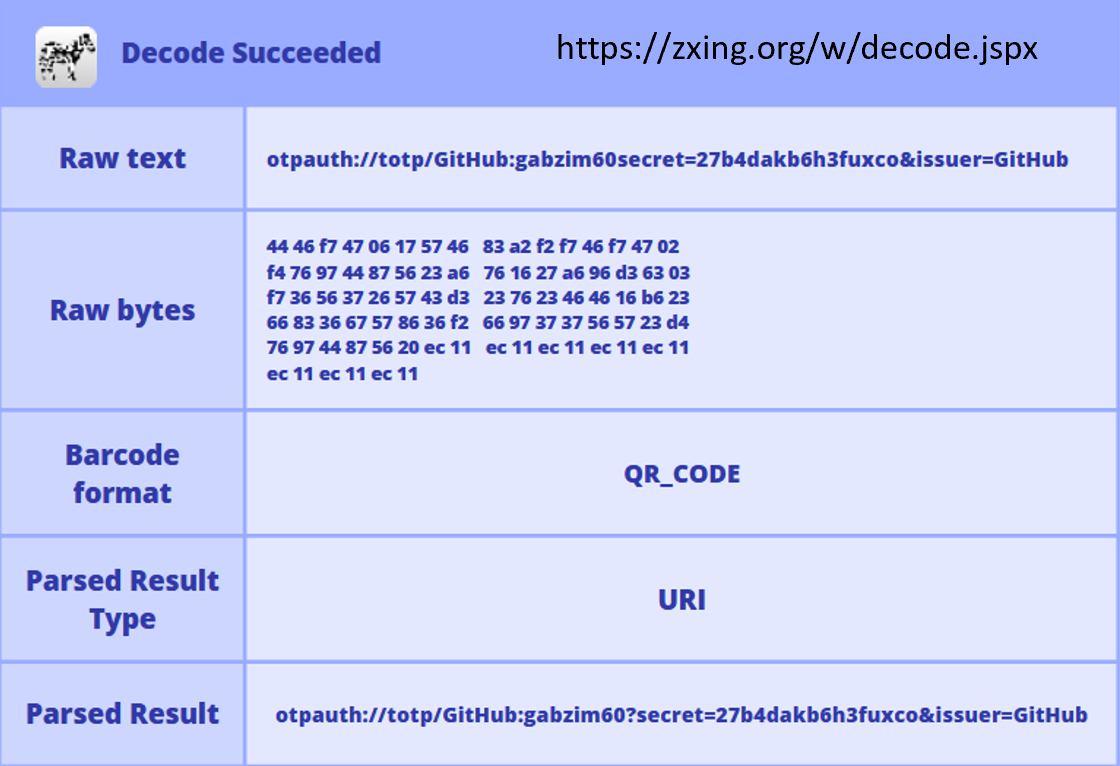
\includegraphics[scale=1]{img/1/1/qrcode-content.png}
        \caption{Exemple de QRcode contenant une seed partagé par le serveur\\}
        \label{fig:2fa-qrcode}
\end{figure}


\noindent
Nous pouvons donc en déduire qu'une \textcolor{myblue}{url de partage de seed} pour l'algorithme \otp est constitué des éléments suivants:
\begin{itemize}
    \item un \textbf{protocole} : \textcolor{mygreen}{otpauth://}
    \item la \textbf{variante d'\otp} utilisée : /totp ou /hotp (expliqué dans la partie suivante)
    \item l'\textbf{émetteur} de la seed : dans l'exemple /GitHub:nomUtilisateur
    \item \textbf{deux paramètres} :
        \begin{enumerate}
            \item le \textbf{secret} encodé en base32 : secret=27b4dakb6h3fuxco
            \item le nom de l'\textbf{émetteur} : issuer=Github
        \end{enumerate}
\end{itemize}    





        %% ***** génération et variantes d'otp ***** %%
        \subsection{Génération et variantes d'\otp}

    Maintenant que le client et le serveur possèdent une \textcolor{mygreen}{donné commune}, ils leurs manquent un \textcolor{myblue}{moyen de créer des codes à usage unique} à partir de cette clé privée. Cela est le rôle de la \textcolor{mygreen}{donnée incrémentale}. La valeur de cette donnée dépend de la variante d'\otp choisie.

            \subsubsection{\hotp}
            
    La première variante d'\otp est appelé \hotp 
qui est l'acronyme de \textcolor{myblue}{'\hmac-based \otp'} et qui se traduit par '\otp basé sur \hmac', 
et utilise un \textcolor{mygreen}{compteur} comme donnée incrémentale.

    En effet, à chaque fois que le client génère un \otp il incrémente un compteur, et le serveur fait de même à la réception d'un \otp valide. Le schéma ci-dessous illustre le mécanisme d'authentification en utilisant \hotp.


\begin{figure}[H]
        \centering
        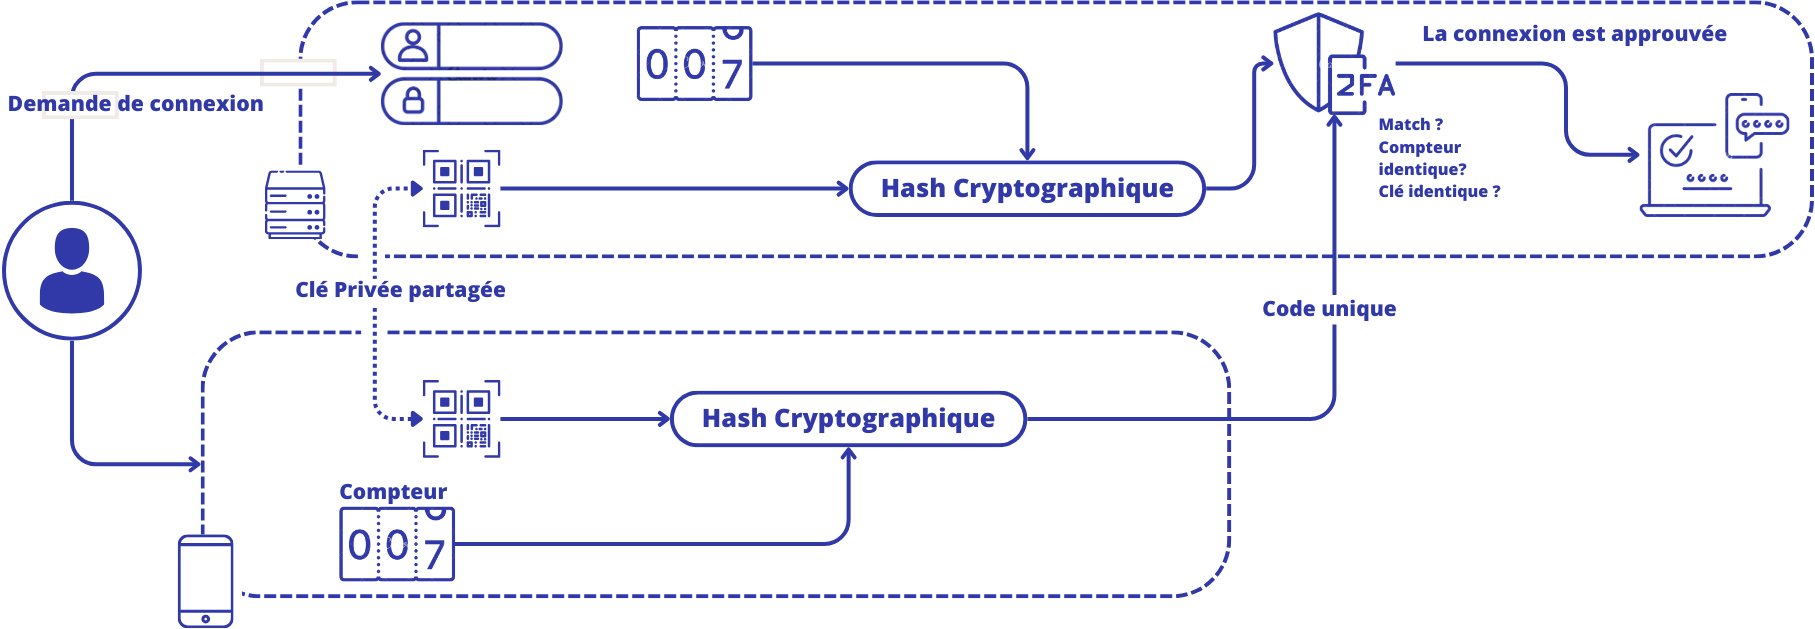
\includegraphics[scale=0.30]{img/1/2/2FA-hotp.png}
        \caption{Expemple 2FA : \hotp\\}
        \label{fig:2fa-hotp}
\end{figure}


Ainsi l'algorithme \hotp nécessite une \textcolor{myblue}{synchronisation constante du compteur} entre le client et le serveur. 
Néanmoins une \textcolor{myblue}{désynchronisation} peut se produire du fait que le client incrémente le compteur à chaque fois qu’il veut créer un code sans savoir s’il a été accepté par le serveur, c’est-à-dire que le serveur à lui aussi incrémenter son compteur.\\

\begin{figure}[H]
        \centering
        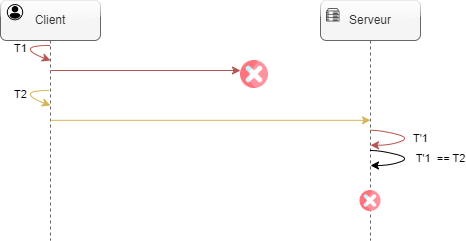
\includegraphics[scale=0.80]{img/1/2/hotp-desync.drawio.png}
        \caption{\hotp : exemple de désynchronisation\\}
        \label{fig:hotp-desync}
\end{figure}

    Pour palier à ce problème, on peut définir un \textcolor{mygreen}{paramètre 'look ahead window'} ('fenêtre d'anticipation' en français) qui permet d'ajuster \textcolor{myblue}{le nombre s de prochaines valeurs} que peux vérifier le serveur afin de \textcolor{mygreen}{détecter les cas de désynchronisation} lorsque le code reçu ne correspond pas au code courant généré. 

\begin{figure}[H]
        \centering
        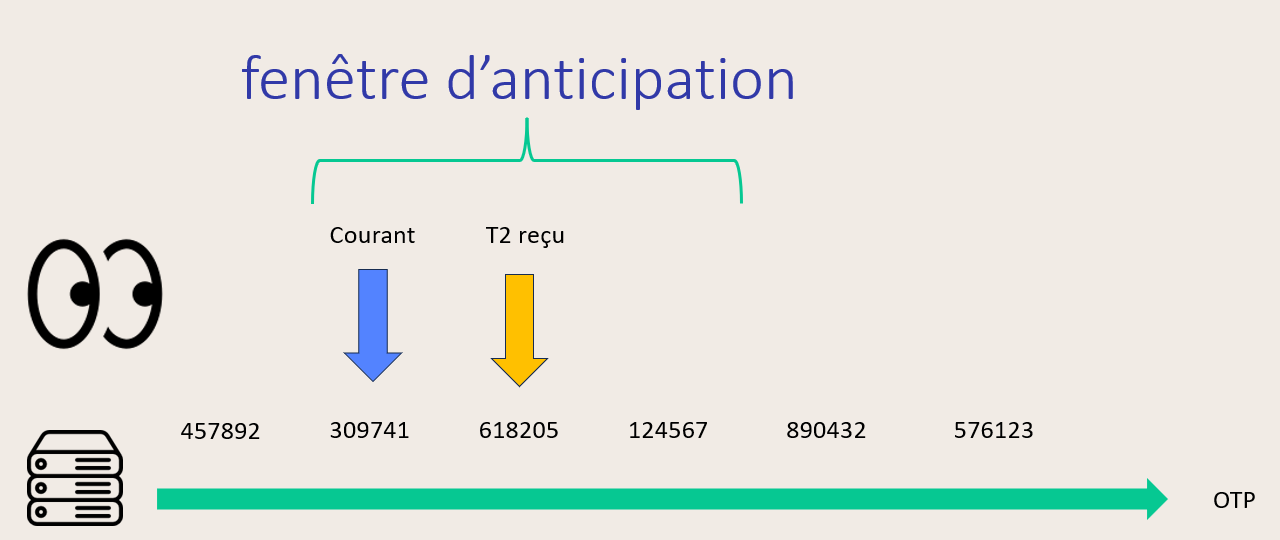
\includegraphics[scale=0.40]{img/1/2/hotp-param-look_ahead_window.png}
        \caption{paramètre \hotp :  look ahead window\\}
        \label{fig:hotp-param-look_ahead_window}
\end{figure}





            \subsubsection{\totp}

    La deuxième variante d'\otp est appelé \totp 
qui est l'acronyme de \textcolor{myblue}{'Time-based \otp'} et qui se traduit par '\otp basé sur le temps'. Il utilise donc un timestamp, plus particulièrement \textcolor{mygreen}{le temps `\textsc{unix}} correspondant au nombre de secondes écoulé depuis le premier janvier 1970, comme donnée incrémentale. 

Le temps \textsc{unix} à été choisi car il est disponible sur la grande majorité des appareils qui tourne sous linux, et en particulier les téléphones mobiles androïde et apple qui sont utilisé dans la plupart des cas.\\

Le \textcolor{myblue}{délai temporel} nécessaire pour générer un nouveau code est généralement fixé à \textcolor{mygreen}{30 secondes} et commence au début d'une nouvelle minute précise. Par exemple, pour les instants de génération, le premier code est associé à 00:00, le deuxième à 00:30, le troisième à 01:00, et ainsi de suite. Ainsi, lorsque l'algorithme doit générer un nouveau code, il \textcolor{myblue}{arrondit le temps vers le bas} jusqu'à l'instant le plus proche marqué par les secondes \textcolor{myblue}{00 ou 30}.


    De ce fait le client et le serveur utilisent le temps courant de leur système arrondis afin de générer un \otp, comme l'illustre le schéma ci-dessous

\begin{figure}[H]
        \centering
        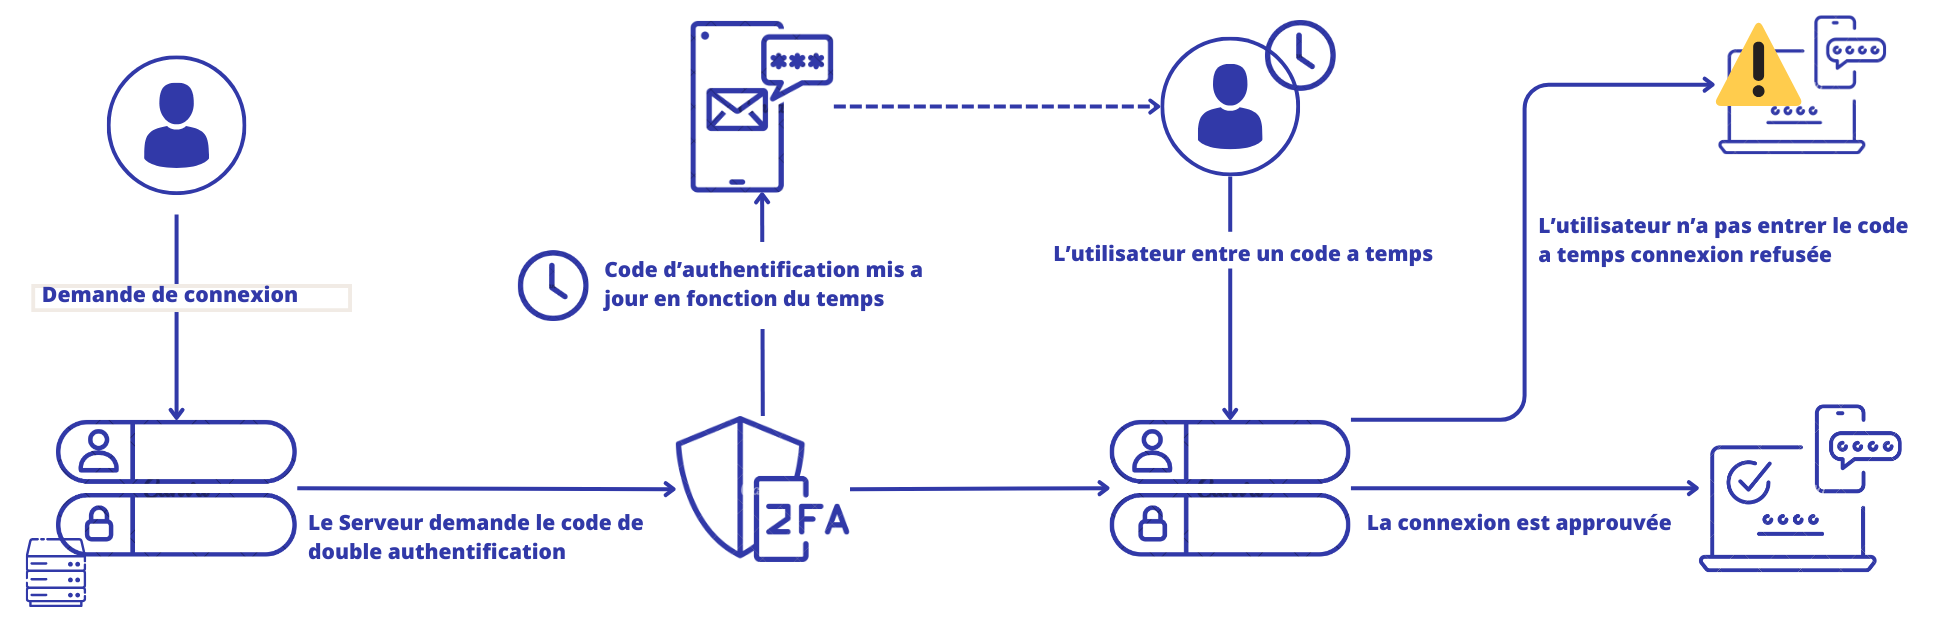
\includegraphics[scale=0.30]{img/1/3/2FA-totp.png}
        \caption{Expemple 2FA : \totp\\}
        \label{fig:2fa-totp}
\end{figure}


    Néanmoins, certains appareils physiques (en particulier dans le domaine des iot) n'ayant pas accès à l'heure d'internet
subissent un \textcolor{myblue}{décalage estimé de deux minutes par an} sans possibilité de réajuster le temps. 
Il peut ainsi être pertinent de configurer un \textcolor{mygreen}{paramètre 'look ahead window'} pour l'utilisation de \totp dans certains \textcolor{myblue}{cas spécifiques.}\\


    Un autre problème rencontré avec l'utilisation de \totp est la \textcolor{myblue}{latence du réseau}. 
En effet, un code valide à son envoie \textcolor{myblue}{n'est pas garantie d'être valide à son arrivé} au serveur suivant le temps mis pour y parvenir, comme illustré dans le schéma ci-dessous.

\begin{figure}[H]
        \centering
        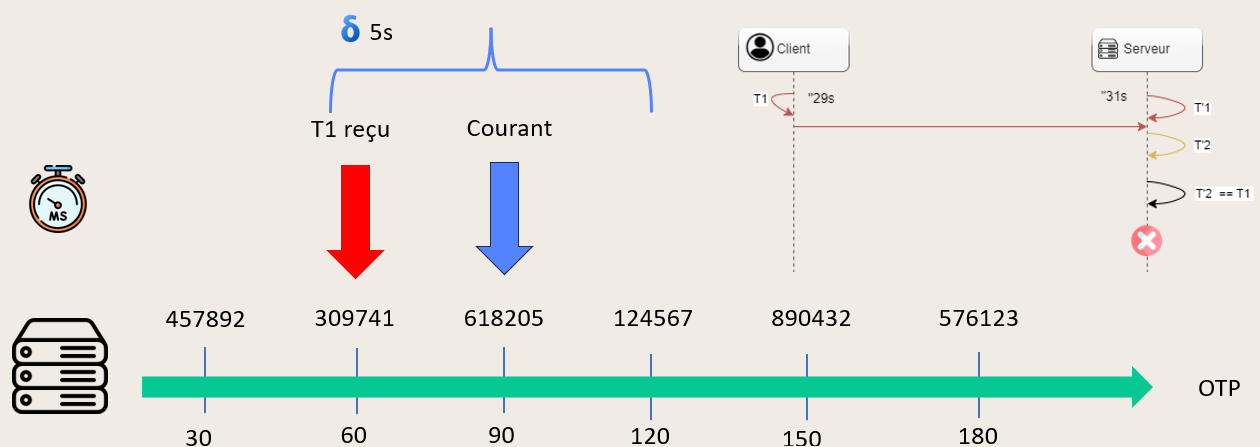
\includegraphics[scale=0.45]{img/1/3/totp_latence.png}
        \caption{\totp: problème de la latence réseau\\}
        \label{fig:totp-latence}
\end{figure}

    
    Ainsi on peut définir une \textcolor{mygreen}{marge temporelle} afin que le serveur compare aussi le code \otp reçus avec le code \otp précèdent
qui rentre dans la marge temporelle, afin de rendre l'utilisation du protocole d'authentification plus fluide pour le client.



        %% ***** gestion de la désynchronisation entre le client et le serveur ***** %%
        \subsection{Gestion de la désynchronisation dans la génération des \otp entre le client et le serveur}


    Une fois que le serveur à \textcolor{myblue}{découvert une désynchronisation} du \otp client reçu avec ceux qu'il a généré dans le 'look-ahead window',
il va aligner son compteur en mémoire avec celui du client et \textcolor{mygreen}{enclencher le protocole de resynchronisation} qui consiste à \textcolor{mygreen}{demander n \otp consécutifs}
afin de s'assurer que le client possède bien la clé secrète et que ce n'étais pas une déduction du code.
    
    Augmenter n va permettre de réduire le succès des attaques de type de brute-force,
mais va rallonger le processus de resynchronisation. Ce paramètre n est \textcolor{mygreen}{en général fixé à 3}.

\begin{figure}[H]
        \centering
        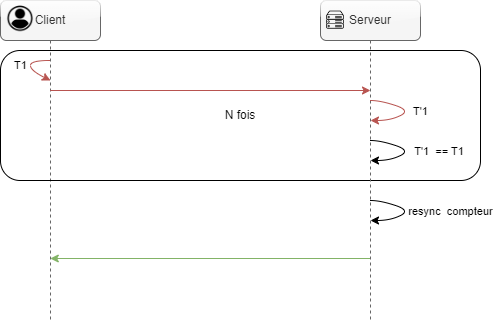
\includegraphics[scale=0.5]{img/1/4/otp-resync.drawio.png}
        \caption{\hotp: resynchronisation du compteur entre le client et le serveur\\}
        \label{fig:hotp-resync}
\end{figure}


    Finalement, si la \textcolor{myblue}{resynchronisation est un succès}, c'est à dire les n codes généré par le client ont été validés par le client, 
le serveur peut \textcolor{mygreen}{mettre à jour son compteur} par rapport au dernier \otp reçu.

Dans le cas où la \textcolor{myblue}{resynchronisation est un échec} le serveur ne met pas son compteur à jour et \textcolor{mygreen}{attend de nouveau un \otp}
jusqu’à ce que la limite fixée par le \textcolor{mygreen}{paramètre d’étranglement soit atteinte}.

Une fois cette limite atteinte, le serveur n'accepte plus d'\otp pour ce compte et le bloque avant d'en notifier le propriétaire qu'une
attivité suspecte de connexion a été détectée.





        %% ***** authentification bi-directionnelle ***** %%
        \subsection{Utilisation d'\otp dans une authentification bi-directionnelle}

    Il est intéressant de noter que l'utilisation d'\otp peut aussi permettre d'effectuer une \textcolor{myblue}{authentification bidirectionnelle}
permettant au client et au serveur de  \textcolor{mygreen}{vérifier leurs identités mutuellement}. 

En effet, en vérifiant chacun leurs tour un \otp reçue de l'autre partie, ils vont chacun pouvoir \textcolor{myblue}{attester de la connaissance
de la clé privé par chacun}.

Ce protocole d'authentification bi-directionnelle se compose donc des étapes suivantes 
(en supposant que le client et le serveur ne présente pas de problèmes de synchronisation traités ci-dessus) :
\begin{enumerate}
    \item Le client génère \textcolor{red}{OTP-C1} et l'envoie au serveur
    \item Le serveur reçoit \textcolor{red}{OTP-C1} et génère \textcolor{red}{OPT-S1},
    \item Le serveur compare \textcolor{red}{OPT-C1} et \textcolor{red}{OPT-S1} :
        \begin{itemize}
            \item si égalité, alors génère \textcolor{yellow}{OPT-S2} et l'envoie au client,
            \item sinon stop le processus.
        \end{itemize}
    \item Le client reçoit\textcolor{yellow}{ OPT-S2} et génère \textcolor{yellow}{OPT-C2},
    \item Le client compare \textcolor{yellow}{OPT-C2} et \textcolor{yellow}{OPT-S2} :
        \begin{itemize}
            \item si égalité, alors vérification terminé, le client \textcolor{teal}{utilise le serveur},
            \item sinon, le client stop le processus.\\
        \end{itemize}
\end{enumerate}

\begin{figure}[H]
        \centering
        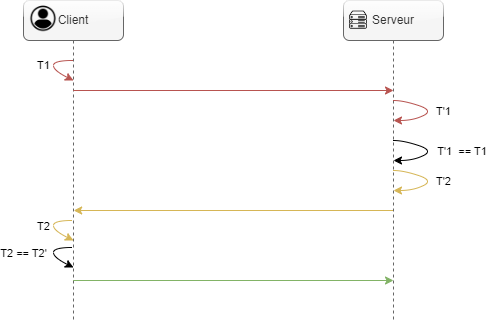
\includegraphics[scale=0.5]{img/1/5/auth-bi-dir.drawio.png}
        \caption{protocole d'authentification bi-directionnelle basé sur \otp}
        \label{fig:hotp-resync}
\end{figure}



\newpage
% ***************************************%
%  2. Algorithme de génération d'OTP     %
% ***************************************%
    \section{Algorithme de génération d'\otp}

\noindent\ L'algorithme de génération d'\otp se compose des quatre étapes suivantes :
    \begin{enumerate}
        \item La gestion d'une \textbf{'seed'} par client permettant de généré des codes pseudo-aléatoires,
        \item Le choix d'une \textbf{donnée incrémentale},
        \item La paramétrisation d'une \textbf{méthode de cryptographie} nommé \hmac,
        \item La \textbf{troncation} de la sortie du \hmac pour obtenir un code à la longueur souhaité.\\
    \end{enumerate}

    Chacune des sous parties de cette section traitera donc d'une partie de cet algorithme afin d'en détailler tous les rouages et de comprendre les enjeux de sécurité liés à chacun d'entre eux.

    %% ***** Gestion de la seed ***** %%
    \subsection{Gestion de la seed}

    La seed est une \textcolor{myblue}{donnée privée} connu uniquement du client et du serveur dont la \textbf{\textcolor{myblue}{création}}, la \textbf{\textcolor{myblue}{communication}} et le \textbf{\textcolor{myblue}{stockage}} vont être des points critiques à la \textcolor{mygreen}{sécurité de l’algorithme}. 
Il est conseillé de prendre une \textcolor{myblue}{clé de même taille que la sortie de la fonction de hachage} utilisée par la méthode \hmac pour garantir l’\textcolor{mygreen}{interopérabilité} entre les systèmes, 
c'est à dire utilisé une taille fixe qui ne dépend pas de la représentation d'un type (int, float, char, ...) faîte par un système et ainsi limiter les problèmes de compatibilité
sous-jacent.

Voici des exemple de taille de clé conseillé selon la fonction de hachage donnée en paramètre de la méthode \hmac :
\begin{description}
    \item[SHA-1] 160 bits
    \item[SHA-256] 256 bits
    \item[SHA-512] 512 bits    
\end{description}


            % == Création == %%
            \subsubsection{Création}

\noindent
Pour générer la seed on a le choix entre deux méthodes :
\begin{gitemize}
    

    \item la génération \textcolor{myblue}{\textbf{aléatoire}}
    \item la génération \textcolor{myblue}{\textbf{déterministe}}
\end{gitemize}


\paragraph*{Génération aléatoire\\}

Cette première méthode est divisée en 2 catégories selon les outils utilisés pour la génération de l’aléatoire.

Ainsi les générateurs s’appuyant sur l’aléatoire d’un \textcolor{mygreen}{phénomène physique} comme par exemple un oscillateur ou un capteur environnemental sont désignés sous le terme \textbf{\textcolor{myblue}{‘hardware-based generator’}}.

Tandis que les générateurs basés sur des \textcolor{mygreen}{algorithmes de pseudo-aléatoire} comme le LFRS (Linear Feedback Shift Register) sont désignés sous le terme \textbf{\textcolor{myblue}{‘software-based generator’}}.


\paragraph*{Génération déterministe\\}

La deuxième méthode est elle aussi divisé en deux catégories.

Soit on va utiliser une \textcolor{myblue}{unique Master Key} \textcolor{mygreen}{($MK$)} générée avec une méthode évoquée précédemment afin d’en \textcolor{myblue}{dériver une seed} pour chaque client,
en utilisant une \textcolor{mygreen}{donnée publique} de ce dernier comme par exemple un numéro de série \textcolor{mygreen}{($i$)}.
La seed est ensuite calculé en faisant un XOR entre la master key et la donnée client, puis en calculant le hash de cette valeur.
\textcolor{red}{$$
    k_i = SHA-1(MK \oplus i)
$$}

Soit on utilise \textcolor{myblue}{une Master Key par client} \textcolor{mygreen}{($MK_i$)} et on utilise également une donnée \textcolor{mygreen}{$j$} du client pour \textcolor{myblue}{dériver une seed}.
Chaque appareil est donc associé à un couple \textcolor{mygreen}{$(i,j)$} afin de retrouver la seed associée.
\textcolor{red}{$$
k_{ij} = SHA-1(MK_i \oplus j)
$$}

            % == Communication == %%
            \subsubsection{Communication}

En ce qui concerne la \textcolor{myblue}{transmission de la seed} du serveur au client, il est impératif d'opter pour un \textcolor{myblue}{canal de communication sécurisé} tel que \textcolor{mygreen}{TLS}/\textcolor{mygreen}{SSL}. 
Ce qui est souvent le cas, car \otp est souvent utilisé pour valider une action d'un client ayant déjà établie une connexion sécurisée.


            % == Stockage == %%
            \subsubsection{Stockage de la seed et conseils de sécurité}

Maintenant, en ayant pris connaissance de ces différentes méthodes, on peut se demander laquelle est plus sécurisé ? Cela dépend en fait du besoin.

En effet, si l'objectif est de \textcolor{myblue}{maximiser la sécurité de la clé}, une approche basée sur le matériel (\textcolor{mygreen}{hardware-based}) est préférable, car elle est \textcolor{myblue}{difficilement prédictible}. Cependant, cette assertion pourrait être remise en question avec l'émergence des ordinateurs quantiques, capables de modéliser l'aspect quantique des phénomènes réels... 

Pour une \textcolor{myblue}{méthode déterministe}, l'utilisation d'\textcolor{mygreen}{une clé maître par client est préférable}, car si une clé est compromise, cela ne compromet pas l'ensemble des seeds des clients.

D'un autre côté, si l'objectif est de \textcolor{myblue}{maximiser la sécurité du stockage} de la clé, il est préférable d'adopter une \textcolor{myblue}{méthode avec une ou plusieurs clés maîtres}. Cela \textcolor{mygreen}{évite le stockage direct de la seed} sur le serveur, contrairement à la méthode aléatoire, qui nécessite le stockage de la clé chiffré par un algorithme symétrique car sa génération n'est pas reproductible.

En ce qui concerne le \textcolor{myblue}{stockage de la clé} avec un algorithme cryptographique symétrique l'\textcolor{mygreen}{AES} est fréquemment utilisé.

\noindent
Pour \textbf{renforcer la sécurité}, plusieurs stratégies peuvent être adoptées :

\begin{itemize}
    \item Utilisation de la \textcolor{myblue}{méthode de Shamir} : Diviser la clé en plusieurs morceaux et les stocker de manière indépendante, éventuellement sur des serveurs distincts. Cela augmente la sécurité du stockage en rendant la récupération complète de la clé plus complexe.

    \item Utilisation de \textcolor{myblue}{données difficiles à obtenir} pour la clé du client : Intégrer des informations telles que le \textcolor{mygreen}{mot de passe chiffré de l'utilisateur}, son numéro de téléphone, ou un calcul d'identifiant basé sur plusieurs données de l'utilisateur. Ceci crée un "secret partagé composite" (composite-shared secret), augmentant la complexité pour un attaquant de compromettre la sécurité.
\end{itemize}

    
    %% ***** Donnée incrémentale ***** %%
    \subsection{Choix d'une donnée incrémentale}

    Le choix entre une donnée incrémentale \textcolor{mygreen}{basée sur le temps}, comme le \totp, ou sur \textcolor{mygreen}{un compteur}, comme le \hotp, dépend des exigences spécifiques de chaque application. 
Dans des contextes où la \textcolor{myblue}{synchronisation temporelle est critique}, le \textcolor{mygreen}{\totp} est avantageux, garantissant la validité temporelle des codes. 
À l'inverse, lorsque \textcolor{myblue}{la séquentialité des actions est plus pertinente}, le \textcolor{mygreen}{\hotp} est préférable, générant des codes uniques en fonction d'un compteur indépendamment du temps. Ainsi, la décision repose sur les caractéristiques particulières du système, les contraintes temporelles et \textcolor{myblue}{les besoins de sécurité spécifiques à chaque scénario d'utilisation}.



    %% ***** HMAC***** %%
    \subsection{Utilisation de \hmac}

        %== définition ==%
        \subsubsection{Définition}

Avec les deux données précédentes (\textcolor{mygreen}{seed}, \textcolor{mygreen}{compteur}), une \textcolor{myblue}{fonction cryptographique} appelée \textcolor{myblue}{\hmac} est employée pour calculer un hash à l'aide d'une fonction telle que SHA-256.
Contrairement à un simple hachage XOR du message et de la clé, \hmac \textcolor{mygreen}{modifie ces deux valeurs avant de les hacher}.\\

\noindent
Voici le \textbf{processus général} de la fonction \hmac :

\begin{enumerate}
    \item Dans un premier temps, on compare la \textbf{taille de la clé} avec la \textbf{taille du bloc d'entrée} de la fonction de hachage, et
    \begin{enumerate}
        \item Si elle est plus grande, on la hache afin d'obtenir une clé de la bonne taille.
        \item Si elle est plus petite, on la complète par des zéros.
    \end{enumerate}
    Cela nous donne la clé effective.

    \item On va ensuite XORer la clé effective avec l'$iPad$ (aussi appelé \textcolor{myblue}{constante de remplissage interne}), qui est une séquence binaire de la même taille donnée en paramètre de \hmac (souvent \texttt{0x36} répété x fois pour remplir le bloc), ce qui donne $R_0$.

    \item Ensuite, on \textbf{concatène} le message à la fin de $R_0$ pour obtenir $R_1$. Puis, on applique la fonction de \textbf{hachage} sur le résultat précédent pour obtenir $H-1$.

    \item Ensuite, on XORe la clé effective avec l'$oPad$ (aussi appelé \textcolor{myblue}{constante de remplissage externe}, souvent \texttt{0x5C}), ce qui donne $R_2$.

    \item On \textbf{concatène} ensuite $R_2$ et $H_1$. Et enfin, on applique la fonction de \textbf{hachage} sur ce résultat pour obtenir le résultat du \hmac.
\end{enumerate}

(NB : ici, on utilise une fonction de \textcolor{myblue}{hachage par bloc} et non linéaire)

\begin{figure}[H]
        \centering
        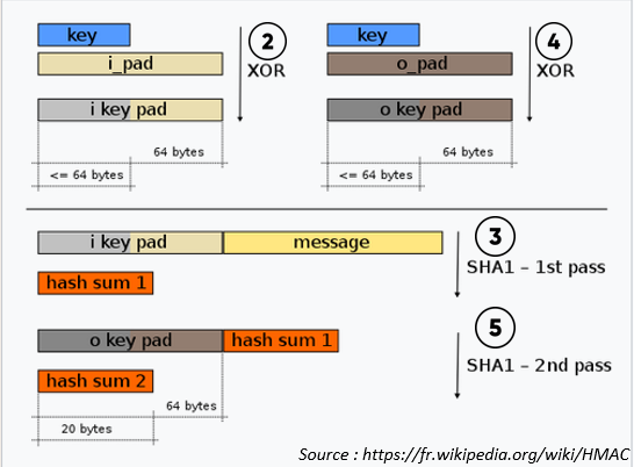
\includegraphics[scale=0.4]{img/2/hmac-wiki.png}
        \caption{schéma de la page wikipédia de hmac}
        \label{fig:hotp-resync}
\end{figure}

\emph{}

        %== Exemple ==%
        \subsubsection{Exemple d'utilisation concret}

\noindent
Pour des raisons de clarté, nous ferons les \textbf{ hypothèses suivantes} dans notre exemple :
\begin{itemize}
    \item La taille du bloc de données est de 8 bits.
    \item La taille de la clé est de 16 bits.
    \item Les constantes $iPad$ et $oPad$ sont respectivement \texttt{0x36} et \texttt{0x5c}, répétées pour remplir le bloc.\\
\end{itemize}

\noindent
Supposons une clé effective de \textcolor{mygreen}{\texttt{0xABCD}}, un compteur de \textcolor{mygreen}{\texttt{0x1234}}, et un message de \textcolor{mygreen}{\texttt{0x5678}}. En utilisant SHA-256 comme fonction de hachage, les constantes $iPad$ et $oPad$ de \texttt{0x36} et \texttt{0x5C} respectivement, le processus serait le suivant :\\
\begin{enumerate}
    \item \textbf{Ajustement de la Clé :} La clé effective reste \texttt{0xABCD}.\\
    \item \textbf{Calcul de $R_0$ :} $R_0 = clé \oplus iPad =$ \texttt{0xABCD} $\oplus$ \texttt{0x36363636} = \texttt{0x36369dfb}.\\
    \item \textbf{Concaténation et Hashing :} $h_1=$SHA-256(\texttt{0x36369dfb5678})=\\
        \texttt{0xbf72f9508c996418e086a5cb96e2399c92fde8a8dde7e1199fad265cf7323d3a}
        \\
    \item \textbf{Calcul de $R_2$ :} $R_2$ = clé $\oplus oPad$ = \texttt{0xABCD} $\oplus$ \texttt{0x5C5C5C5C} = \texttt{0x5c5cf791}.\\
    \item \textbf{Finalisation du \hmac :} Concaténation de $R_2$ et $H_1$, puis application de SHA-256 pour obtenir le résultat final du \hmac :\\
    \hmac = SHA-256($r_2 \oplus H_1$) =\\
    = SHA-256(\texttt{0x5c5cf791bf72f9508c996418e086a5cb96e2399c92fde8a8dde7e1199fad265cf7323d3a})\\
     = \texttt{0x349808a3963b903444dc6cad5ffd5b11ff7a8edd42d244a605ffe0ee806250e2}\\
\end{enumerate}

\noindent
Cet exemple illustre le processus HMAC avec des \textbf{valeurs concrètes} et les \textbf{constantes spécifiées}.


    
    %% ***** troncation ***** %%
    \subsection{Troncation de la sortie du \hmac}

        %== définition ==%
        \subsubsection{Définition}

Une fois le \textcolor{myblue}{\hmac calculé}, il est nécessaire de le \textcolor{myblue}{tronquer} pour obtenir un code de la longueur souhaitée.
Pour ce faire, nous examinons les \textcolor{mygreen}{4 bits de poids faibles} du \hmac, cette valeur nous \textcolor{mygreen}{fournit l'offset} à partir duquel \textcolor{mygreen}{extraire une portion de 4 bytes}.

Ensuite, pour obtenir l'\otp, nous appliquons le \textcolor{myblue}{modulo de \(10^n\)} pour \textcolor{mygreen}{obtenir un code à \(n\) chiffres}. Avant de calculer le modulo, un \textcolor{myblue}{masque} est appliqué pour obtenir un \textcolor{mygreen}{entier non signé} en big-endian de 31 bits.
Ce processus permet de générer un code \otp de la longueur spécifiée à partir du HMAC calculé.


        %== Exemple ==%
        \subsubsection{Exemple d'utilisation concret}

Reprenons le résultat du \hmac de notre exemple, et tronquons le pour le transformer en \otp de 6 chiffres :

\begin{center}
\begin{tabular}{|c c c c c c c c c c c c c c c c c|}
\hline
Index & 0 & 1 & \color{red}{2} & \color{red}{3} & \color{red}{4} & \color{red}{5} & 6 & 7 & 8 & 9 & 10 & 11 & 12 & 13 & 14  & 15\\
\hline
Valeur & 34 & 98 & \color{green}{08} & \color{green}{a3} & \color{green}{96} & \color{green}{3b} & 90 & 34 & 44 & dc & 6c & ad & 5f & fd & 5b & 11\\
\hline 
\hline
Index  & 16 & 17 & 18 & 19 & 20 & 21 & 22 & 23 & 24 & 25 & 26 & 27 & 28 & 29 & 30 & 31\\
Valeur  & ff & 7a & 8e & dd & 42 & d2 & 44 & a6 & 05 & ff & e0 & ee & 80 & 62 & 50 & e2\\
\hline
\end{tabular}
\end{center}

\noindent

Ici les 4 bits de poids faible sont \textbf{\texttt{0x2}} ce qui nous donne \textbf{l'index 2} à partir duquel on extrait les 4 bytes suivant : \textbf{\texttt{0x08a3963b}} qui équivaut à \texttt{144938555} en base 10.

On calcule ensuite le modulo 6 de cette valeur : $ 144938555 \text{ mod } 10^6 = $ \textbf{938\ 555}, ce qui correspond à notre \otp !








\newpage
% *******************************************%
%  3. Prototype python de l'algorithme OTP   %
% *******************************************%
    \section{Prototype python de l'algorithme \otp}

    Afin de \textcolor{myblue}{mieux comprendre les concepts} expliqués dans la partie précédente et de mesurer les différents enjeux de sécurité discutés dans la première partie, nous avons décidé de réaliser une \textcolor{myblue}{implémentation de l'algorithme \otp dans le cadre du 2FA}.

    Pour réaliser ce prototype nous avons choisi d'utiliser \textcolor{mygreen}{python} et la \textcolor{mygreen}{librairie flask} pour le frontend. Dans un premier temps, La librairie \textcolor{mygreen}{pyotp} qui implémente l'algorithme \otp a été utilisé pour accélérer le développement, puis nous avons décider de créer \textbf{\textcolor{mygreen}{notre propre implémentation de l'algorithme \otp}} selon les étapes expliqués dans la partie précédente.\\

    Cette section vise donc à expliquer les \textbf{choix de conceptions} réalisés pour l'implémentation de l'algorithme et de montrer au lecteur comment \textcolor{myblue}{mettre en place une authentification à double facteurs} dans une application, dont les captures d'écran des différentes pages peuvent être consulté dans l'annexe-\ref{ann:app}.



    %% ***** architecture ***** %%%
    \subsection{Architecture et déploiement}

    Notre implémentation du protocol \otp se constitue d'une \textcolor{mygreen}{application web} réalisée avec la librairie Flask de python. La Figure-\ref{fig:proto-archi} représente l'arborescence des fichiers de ce projet. Le serveur '\textcolor{mygreen}{gunicorn}' a été sélectionné afin de déployer l'application sur Heroku à l'addresse \textbf{\url{https://dsc-securite-otp-c9eac3f8716a.herokuapp.com/}}.\\

\noindent
Le dossier '/app' contient le code source de l'application organisé comme suit :
\begin{description}
    \item[app.py :]
    Ce fichier est le point d'entrée de l'application et contient la \textcolor{myblue}{création et paramétrisation} de cette application, ainsi que les route des url '/'.
    \item[config\_\*.py]
    Ces fichiers contiennent des \textcolor{myblue}{paramètres globaux} de l'application telle que la taille des codes \otp générés.
    \item[helpers.py]
    Ce fichier contient les méthods générales pour créer les pages d'\textcolor{myblue}{affichages d'information} aussi bien pour le serveur que pour le client, ce qui nous permet d'éviter la redondance de code.
    \item[myOTP.py]
    Ce fichier contient l'\textcolor{myblue}{implémentation personnelle} de génération de code \otp\ , c'est à dire les fonctions \textcolor{mygreen}{hmac}, \textcolor{mygreen}{troncation}, et la \textcolor{mygreen}{gestion du pas temporelle} de 30 secondes pour les \totp\ .
    \item[share\_\ seed.py]
    Ce fichier contient les fonctions de \textcolor{myblue}{génération de QRcode} afin de partager la seed à une application comme \textcolor{mygreen}{freeOTP Authenticator-\ref{fig:freeotp}} afin que l'utilisateur puisse générer ses codes sur son propre appareil.
    \item[/client et /server] 
    Ces répertoires contiennent la logique pour les url respectives '/client/' et '/server'.\\
\end{description}

\noindent
Le projet contient aussi des fichiers spécifiques au déploiements listés ci-dessous:
\begin{description}
    \item[.github/workflows/main.yml] 
    Ce fichier constitue notre \textcolor{myblue}{pipeline de déploiement} sur \textcolor{mygreen}{héroku} lors du push dans la branche main de nôtre répot github.
    \item[Procfile] 
    Ce fichier est utilisé par Heroku pour \textcolor{myblue}{lancer l'application}.\\
\end{description}


    %% ***** pyotp ***** %%
    \subsection{Utilisation de pyotp}

La librairie \textbf{pyotp} est utilisé pour générer les seed avec la fonction \textbf{random\_base32} qui selon la documentation effectue un tirage aléatoire dans une liste prédéfinie afin d'obtenir une seed.

\begin{figure}[H]
        \centering
        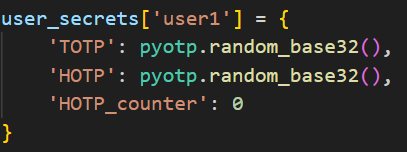
\includegraphics[scale=1]{img/C_proto/code/code_pyotp_seed.png}
        \caption{Génération d'une seed en base32 avec pyotp\\}
        \label{fig:code-seed}
\end{figure}

    
    %% ***** implémentation personnelle ***** %%
    \subsection{Implémentation personnelle de l'algorithme \otp}

Cette section présente une \textbf{capture d'écran des fonctions implémentées} pour la réalisation d'un algorithme générant des \totp et \hotp en python afin de les répertoriées dans ce rapport et \textbf{rendre leurs consultation plus accessible}. Ainsi elle n'apportera pas plus d'explication par rapport aux explications précédentes et aux commentaires présent dans le code.


\begin{figure}[H]
        \centering
        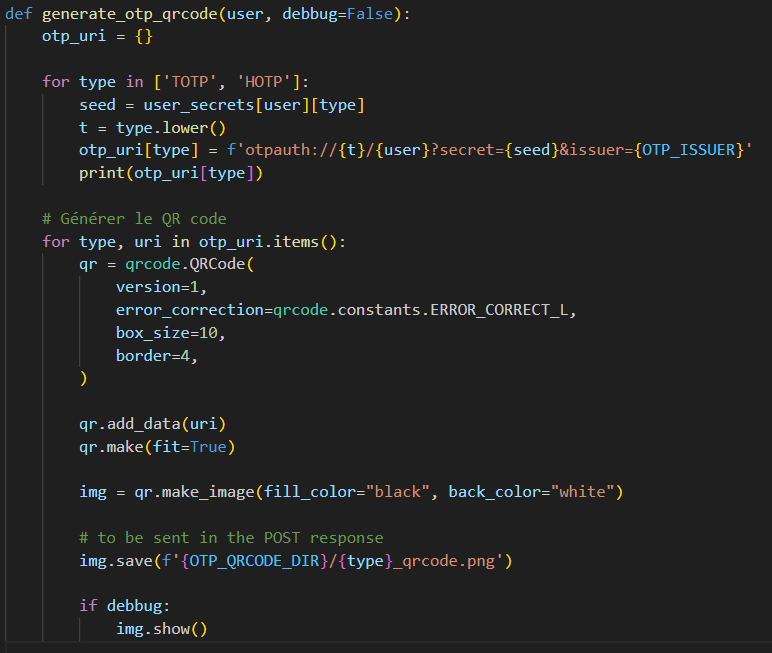
\includegraphics[scale=0.8]{img/C_proto/code/code_share_seed.png}
        \caption{Création d'un uri et d'un QRcode pour le partage de la seed\\}
        \label{fig:code-round-time}
\end{figure}


\begin{figure}[H]
        \centering
        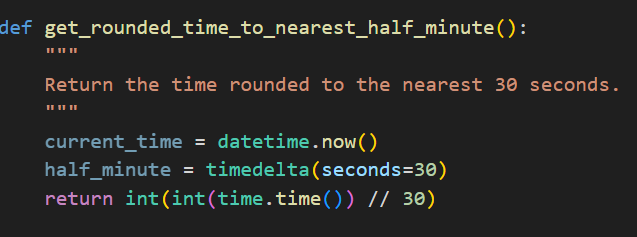
\includegraphics[scale=0.8]{img/C_proto/code/code_round_time.png}
        \caption{arrondissement du temps au multiple de 30s le plus bas\\}
        \label{fig:code-round-time}
\end{figure}

\begin{figure}[H]
        \centering
        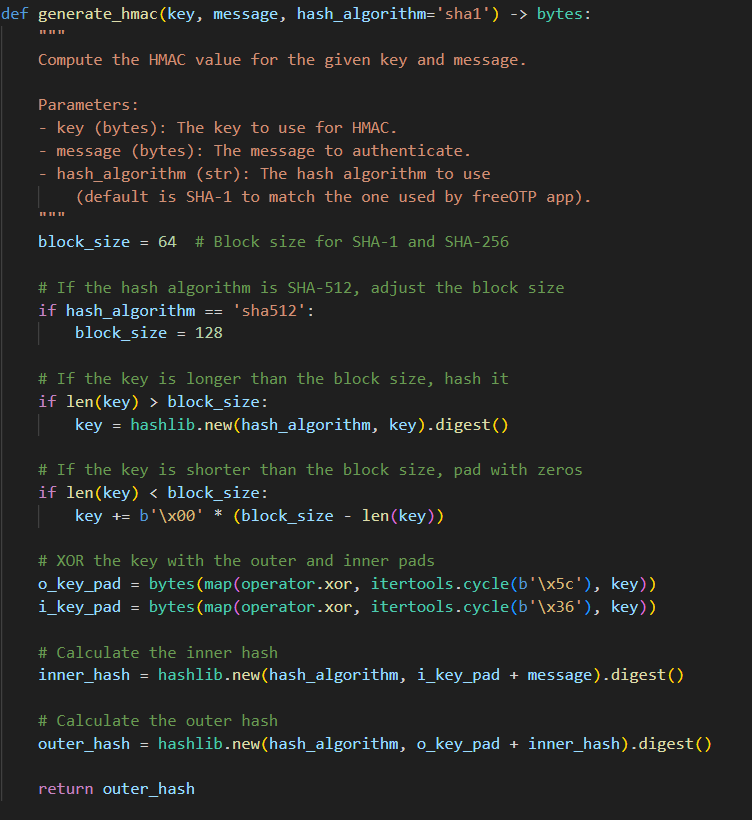
\includegraphics[scale=1]{img/C_proto/code/code_hmac.png}
        \caption{implémentation de \hmac part 1\\}
        \label{fig:code-hmac}
\end{figure}

\begin{figure}[H]
        \centering
        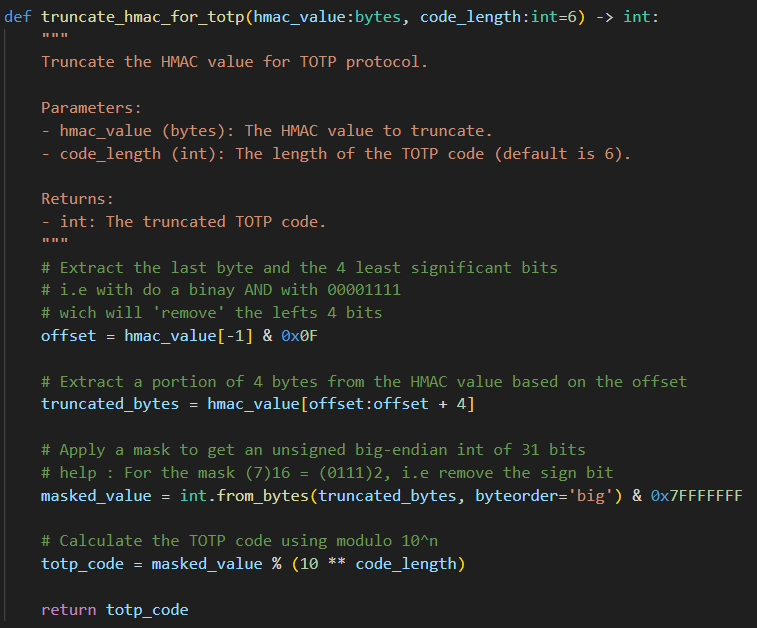
\includegraphics[scale=1]{img/C_proto/code/code_trunc.png}
        \caption{implémentation de \hmac part 2\\}
        \label{fig:code-trunc}
\end{figure}

\begin{figure}[H]
        \centering
        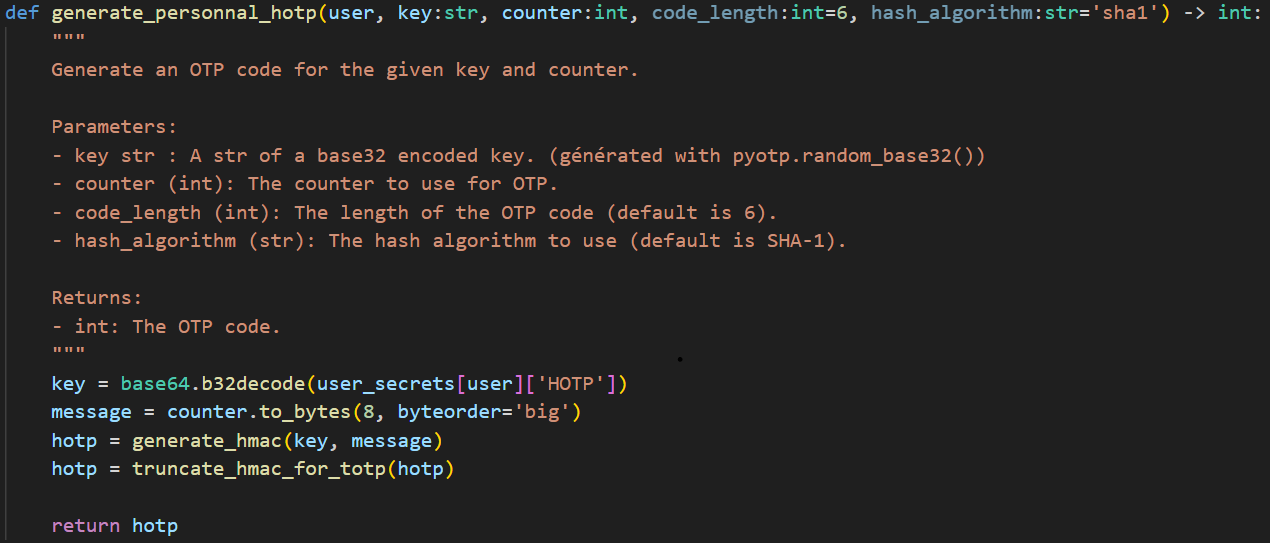
\includegraphics[scale=0.7]{img/C_proto/code/code_hotp.png}
        \caption{implémentation de \hotp\\}
        \label{fig:code-hotp}
\end{figure}

\begin{figure}[H]
        \centering
        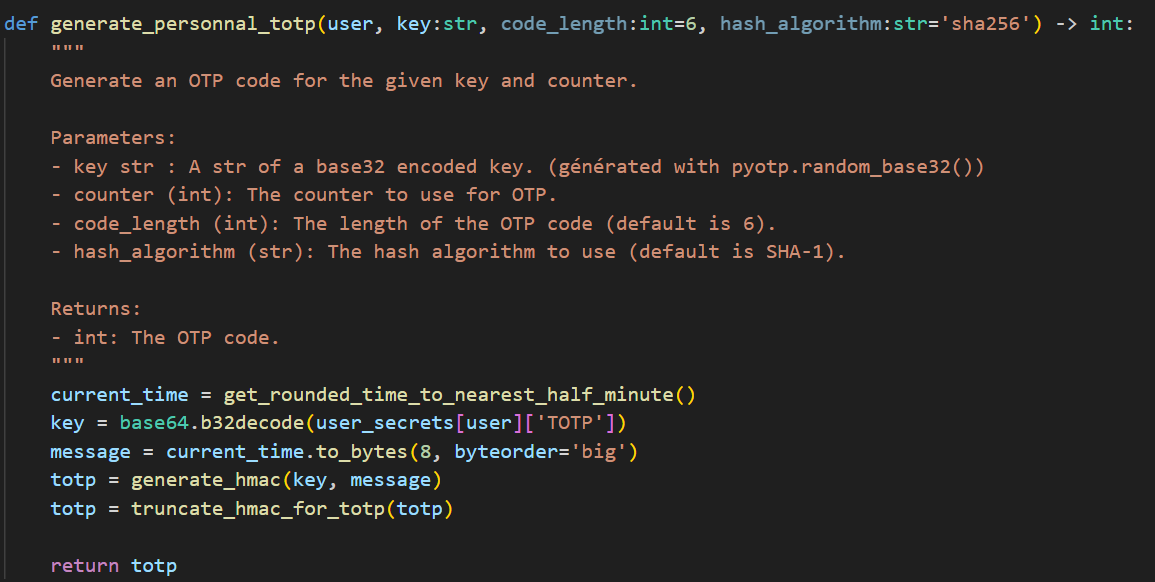
\includegraphics[scale=0.7]{img/C_proto/code/code_totp.png}
        \caption{implémentation de \totp\\}
        \label{fig:code-totp}
\end{figure}



\begin{figure}[H]
        \centering
        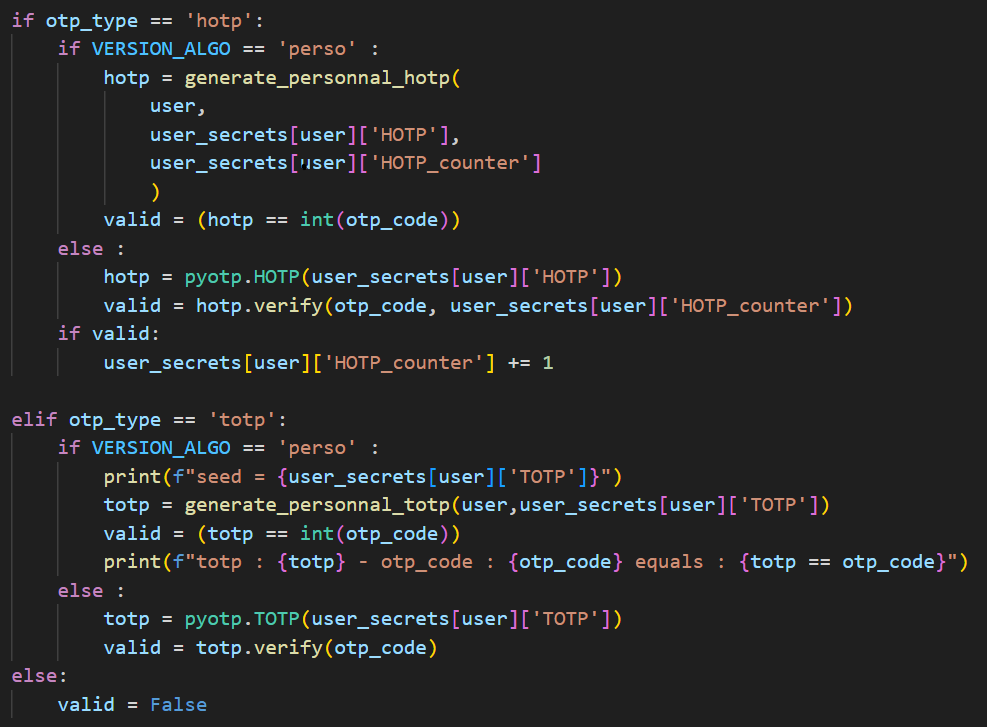
\includegraphics[scale=0.7]{img/C_proto/code/code_val_otp.png}
        \caption{Serveur comparaison d'un \otp reçu}
        \label{fig:code-val}
\end{figure}


    
    %% ***** mise en place du 2FA ***** %%
    \subsection{Mise en place du 2FA dans une application}

    Pour conclure, afin de \textcolor{myblue}{mettre en place un protocole 2FA} dans une application vous pouvez suivre les étapes suivantes :
\begin{enumerate}
    \item Trouvez une fonction de \textbf{génération de seed} aléatoire,
    \item Utilisez une librairie de \textbf{génération de QRcodes} pour partager la seed grâce au format d'uri suivant : \\
            \textcolor{mygreen}{otpauth://\{totp, hotp\}/\{username\}?secret=\{seed\_base32\_encoded\}\&issuer=\{issuer\_name\}} ;\\
            et ainsi permettre à l'utilisateur de générer des \otp avec son application favorite.
    \item utilisez une librairie de \textbf{générateur d'\otp} ou implémentez les fonctions ci-dessus
    \item à la connexion, après que l'utilisateur a rentré son nom et mot de passe, affichez une pop-up pour \textbf{vérifier le code} \otp\ .
    \item du côté du serveur, à la réception d'un code \otp générez un \otp en fonction de la seed de l'utilisateur et du temps ou du compteur de l'utilisateur afin de \textbf{vérifier la validité de l'\otp reçue} et \textbf{valider l'action} d'authentification.
\end{enumerate}









\newpage
% *********************************************************%
%  4. Conclusion, failles de sécurité et bonnes pratiques  %
% *********************************************************%
    \section{Conclusion : failles de sécurité et bonnes pratiques}

Pour conclure, \otp est largement adopté et \textcolor{myblue}{utilisé pour valider des actions} tels que l’authentification ou des transactions, mais \textbf{ne garantit pas une sécurité optimale} si on ne prend pas des précautions
\begin{itemize}
    \item	Faille sécurité partage de la seed
    \item	Faille pour le partage via SMS/mail (fishing, interception de SMS)
    \item	Code de 6 chiffres => brute force si pas de limite de tmps fixé (généralement double le temps d’attente à chaque code erroné)
    \item	Vols de recovery codes (code donnée à l'utilisateur après l'activation du 2FA pour le bypass avec un de ces codes en cas de perte de sa possession) 
\end{itemize}

Il est donc conseillé de fixer un \textcolor{mygreen}{paramètre d’étranglement} pour limiter le nombre de tentatives autorisées par utilisateur. Ou alors un \textcolor{mygreen}{schéma de délais} pour qu'après chaque tentative de connexion, le serveur attend \textcolor{mygreen}{A*T secondes} pour répondre (T souvent 5s).


On estime la sécurité de l'algorithme \otp mis en place avec la formule suivante :
\textcolor{myblue}{$$
Sec = s * v / 10^Digit
$$}
\noindent
Avec :
\begin{itemize}
    \item[Sec :] probabilité de succès d’une attaque.
    \item[S : ] paramètre de la fenetre d’anticipation (look-ahead window).
    \item[V : ] le nombre de tentatives autorisées.
    \item[Digit : ] le nombre de digit du code OTP.\\
\end{itemize}


Les deux systèmes \otp proposent des codes à usage unique, mais la \textbf{différence essentielle} réside dans le fait que, dans le système \hotp, un \textbf{\hotp} donné est \textbf{valable jusqu'à ce qu'il soit utilisé}, ou jusqu'à ce qu'un \otp ultérieur soit utilisé ce qui crée une vulnérabilité qui peut être utilisée par des attaquants. 

\noindent
Il existe d'autres \textcolor{myblue}{\textbf{vulnérabilités}} plus communes répertoriées dans le tableau suivant :


\begin{table}[H]
\centering
\begin{tabular}{| p{2cm} | p{6cm} | p{8cm} |}
\hline
\textbf{Nom de l'attaque} & \textbf{Déroulement de l'attaque} & \textbf{Défense} \\
\hline
Phishing & Les attaquants trompent les utilisateurs pour obtenir leurs \otp via des e-mails, SMS ou des sites web malveillants. & Sensibilisation des utilisateurs, utilisation d'une authentification à deux facteurs (2FA) avec codes générés depuis une application pour renforcer la sécurité. \\
\hline
Attaque par interception de SMS (SWAP SMS) & Intercepter les \otp envoyés par SMS à l'aide de logiciels malveillants ou de dispositifs de surveillance. & Préférer des méthodes d'\otp ne reposant pas sur les SMS, tels que les applications d'authentification. \\
\hline
Brute Force & Les attaquants essaient différentes combinaisons pour deviner un \otp. & Imposer des politiques de complexité pour les OTP, tels que des codes plus longs et moins prédictibles. Définir un schéma de délais pour limiter le nombre de tentatives et doubler le temps d'attente à chaque erreur. \\
\hline
Attaque par rejeu & Intercepter un \otp valide et le réutiliser pour accéder au compte de l'utilisateur. & Utiliser des mécanismes de protection contre les attaques de rejeu, comme les horodatages. \\
\hline
Vol de clé secrète & Compromission de la clé secrète utilisée pour générer les \otp. & Stockage sécurisé des clés, rotation régulière des clés. \\
\hline
Utilisation d'applications tierces non sécurisées & Stockage ou transmission vulnérable des \otp par des applications tierces. & Utiliser des applications d'authentification reconnues et sécurisées. \\
\hline
Ingénierie sociale & Manipulation des utilisateurs pour divulguer leurs \otp en se faisant passer pour une autorité légitime. & Sensibilisation des utilisateurs, vérification stricte des demandes d'informations sensibles. \\
\hline
\end{tabular}
\caption{Tableau des attaques \otp et des défenses correspondantes}
\label{tab:otp_attacks_defenses}
\end{table}




% En d'autres termes : 
% \begin{itemize}
%   \item Un algorithme est utilisé pour générer un nouveau code aléatoire à chaque fois qu'un mot de passe est nécessaire.Par SMS / e-mail ou une application d'authentification.
%   \item Une fois que le code \otp a été généré, l'utilisateur le copie.
%   \item Le code OTP entré par l'utilisateur est comparé au code généré côté serveur pour vérifier son authenticité.
%   \item Si les codes correspondent, l'utilisateur reçoit un message "Authentifié" et peut accéder à son compte.
%   \item Après avoir été utilisé ou après expiration de sa durée de validité, l'OTP n'est plus valable et ne peut pas être réutilisé. Un nouveau code est généré pour la prochaine authentification.
% \end{itemize}
% \begin{figure}[H]
%         \centering
%         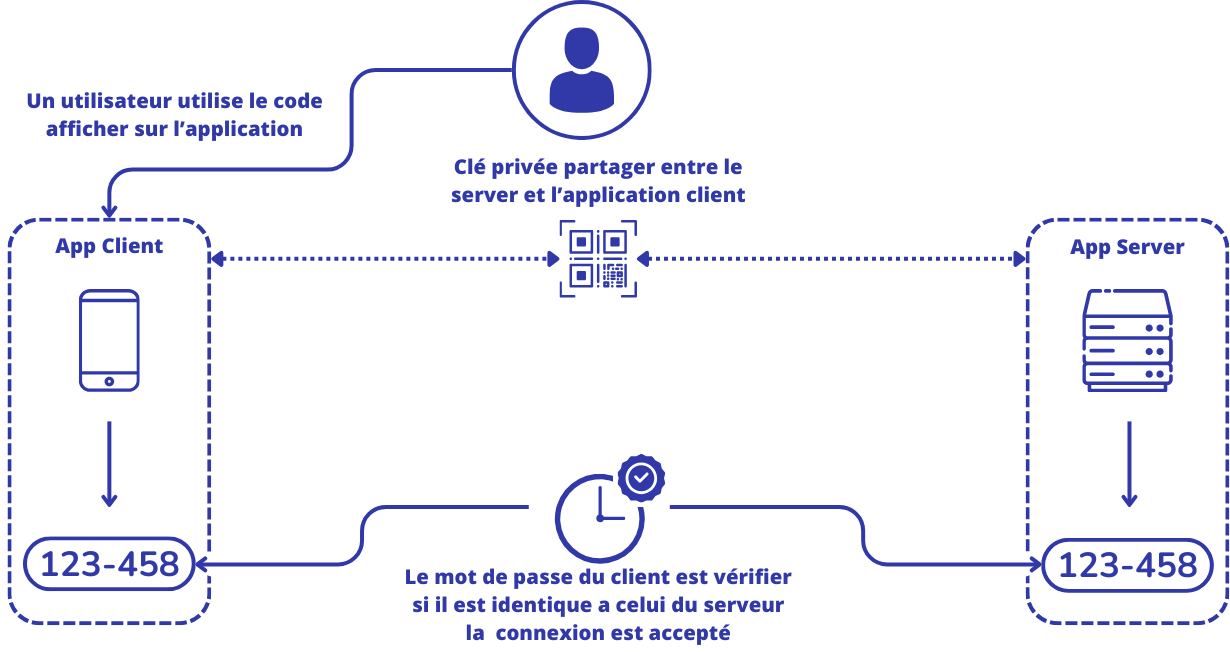
\includegraphics[scale=0.5]{img/introOTP.png}
%         \caption{Schéma Client Serveur}
%         \label{fig:tock_logo}
% \end{figure}
% \section{Cryptographie dans les OTP}
% % \begin{itemize}
% %   \item Aperçu de la cryptographie. HMAC SHA1
% %   \item Rôle de la cryptographie dans la sécurisation des OTP.
% % \end{itemize}
% HMAC SHA1 est appliquée pour sécuriser les messages dans les systèmes OTP. 

% HMAC (Hash-based Message Authentication Code) utilise une combinaison de clé secrète et de fonction de hachage pour authentifier un message. SHA1 (Secure Hash Algorithm 1).

% Bien qu'il est ancien, il est toujours utilisé dans certains systèmes comme les OTP pour le cryptage d'un message. SHA1 génère un résumé de message de 160 bits, afin de garantir que le message ne soit pas altéré. De nos jours, le SHA1 est de moins utilisée il y'a une migration vers des fonctions de hachage plus sécurisées comme SHA256.

% \begin{figure}[H]
%         \centering
%         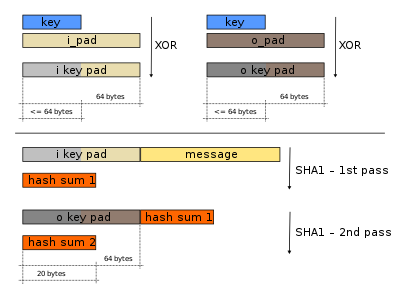
\includegraphics[scale=1]{img/SHAhmac.png}
%         \caption{illustration prise de \url{https://fr.wikipedia.org/wiki/HMAC}}
%         \label{fig:tock_logo}
% \end{figure}


% \newpage
% \subsection{TOTP (Time-based One Time Password)}
% Le TOTP quant a lui, se distingue par son utilisation du temps actuel au lieu d'un compteur pour générer des mots de passe. Pour créer un TOTP, un secret partagé est combiné avec l'heure actuelle, divisée typiquement en tranches de 30 secondes. 

% Ce mélange est alors haché avec une fonction HMAC. L'avantage du TOTP réside dans la courte durée de vie des mots de passe, améliorant ainsi la sécurité en limitant les risques d'utilisation frauduleuse.

% \begin{figure}[H]
%     \centering
%     \includegraphics[scale=0.35]{img/TOTPSchema.png}
%     \caption{Schéma Client Serveur}
%     \label{fig:tock_logo}
% \end{figure}

% \newpage









\appendix
\newpage
\clearpage
\pagenumbering{roman} % Retour à la numérotation arabe pour le reste du document
\setcounter{page}{1} % Réinitialisation du compteur de page à 1

`\section{Vocabulaire}

\begin{center}
    \begin{tabular}{|m{3cm}|m{8cm}|}
        \hline
        \textbf{Vocabulaire} & \textbf{Définition} \\
        \hline
        2FA & double facteur d'authentification : protocole dans lequel un utilisateur doit prouver son identité en fournissant son mot de passe et en donnant un mot de passe généré/communiqué par un moyen que seul lui connaît. \\
         \hline
        AES & Advanced Encryption Standard, algorithme cryptographique symétrique \\
        \hline
        brute-force & attaque visant à tester toutes les combinaisons possibles afin de briser la sécuriter d'un système.\\
        \hline
        hexadécimal & notation en base 16 préfixée par \texttt{0x} chaque chiffre peut prendre une valeur parmis [0-9AF].\\ 
       \hline
        HMAC & Mash Message Authentification Code : génère un code en utilisant une clé secrète, un message et unz fonction de hachage \\
         \hline
        IETF & : Internet Engineering Task Force, défini des standard d’Internet (non officiel), mais suivis par de nombreux dev.\\
        \hline
        iPad & constante de remplissage interne dans la fonction HMAC permettant d'homogénéiser la taille de la clé avec la taille de bloc de la fonction de hash configuré.\\
         \hline
        LFSR & Linear Feednack Shift Registration, algorithme de génération de séquence binaire pseudo-aléatoire. \\
       \hline
        oPad & constante de remplissage externe dans la fonction HMAC permettant d'homogénéiser la taille de la clé avec la taille de bloc de la fonction de hash configuré. \\
       \hline
        \otp & mot de passe à usage unique \\
        \hline
        seed & désigne une séquence servant d'origina à la génération d'une séquence pseudo-aléatoire.\\
       \hline
        XOR & opération binaire qui est vrai quand un seul des 2 bits est vrai.\\
        \hline
        Xorer & effectuer l'opération XOR entre 2 valeurs.\\
        \hline
    \end{tabular}
\end{center}










\newpage
\section{Références}

% Ajuste la hauteur des lignes dans le tableau
\renewcommand{\arraystretch}{2.5}

\begin{tabular}{p{0.5\linewidth}p{0.4\linewidth}}
   \textbf{\totp: Time-Based One-Time Password Algorithm} & \url{https://datatracker.ietf.org/doc/pdf/rfc6238} \\
   
   \textbf{Research Article C-Lock: Local Network Resilient Port Knocking System Based on TOTP} & \url{https://downloads.hindawi.com/journals/wcmc/2022/9153868.pdf} \\
   
   \textbf{Group Time-based One-time Passwords and its Application to Efficient Privacy-Preserving Proof of Location} & \url{https://eprint.iacr.org/2022/1280.pdf} \\
   
   \textbf{\hotp: An HMAC-Based One-Time Password Algorithm} & \url{https://www.ietf.org/rfc/rfc4226.txt} \\
   
   \textbf{Fuites de mots de passe} & \url{https://www.01net.com/actualites/246-milliards-d'identifiants-et-mots-de-passe-voles-circulent-sur-la-toile-les-votres-aussi.html} \\
   
   \textbf{Étude sur la réutilisation de mots de passe} & \url{https://fr.statista.com/statistiques/967863/nombre-mots-de-passe-comptes-en-ligne-france/} \\
   
   \textbf{Génération de secrets aléatoires} & \url{https://datatracker.ietf.org/doc/html/rfc4086} \\
   
   \textbf{Échange de clés} & \url{https://eprints.qut.edu.au/31900/} \\
   
   \textbf{Word list to make seed phrase} & \url{https://github.com/bitcoin/bips/blob/master/bip-0039/bip-0039-wordlists.md} \\
   
   \textbf{Article intéressant sur Medium} & \url{https://medium.com/@nicola88/two-factor-authentication-with-totp-ccc5f828b6df} \\
   
   \textbf{Code source d'une application d'authentification} & \url{https://freeotp.github.io/} \\
   
   \textbf{Vidéo sur \hotp \& \totp} & \url{https://www.youtube.com/watch?v=XYVrnZK5MAU&list=PL3xlPfx1FbdbMafMn6sD3d3KEL3pGMpI7&index=2&t=7s} \\
   
   \textbf{Vidéo sur \totp} & \url{https://www.youtube.com/watch?v=VOYxF12K1vE&list=PL3xlPfx1FbdbMafMn6sD3d3KEL3pGMpI7&index=3&t=792s} \\
   
   \textbf{Tutoriel vidéo sur pyotp} & \url{https://www.youtube.com/watch?v=o0XZZkI69E8&list=PL3xlPfx1FbdbMafMn6sD3d3KEL3pGMpI7&index=4&t=391s} \\
   
   
\end{tabular}

\begin{tabular}{p{0.5\linewidth}p{0.4\linewidth}}
    \textbf{Vidéo sur l'\otp envoyé par un fournisseur (SMS/email) n'est pas sécurisé} & \url{https://www.youtube.com/watch?v=o0XZZkI69E8&list=PL3xlPfx1FbdbMafMn6sD3d3KEL3pGMpI7&index=4&t=391s} \\
     \textbf{Vidéo sur TOTP et la vie privée des données} & \url{https://www.youtube.com/watch?v=ChKpf5HjcSY&list=PL3xlPfx1FbdbMafMn6sD3d3KEL3pGMpI7&index=6&t=1143s} \\
   
   \textbf{Étude vidéo sur Google Authenticator} & \url{https://www.youtube.com/watch?v=2vP0gT5wGlA&list=PL3xlPfx1FbdbMafMn6sD3d3KEL3pGMpI7&index=7} \\
   
   \textbf{Vidéo sur les attaques sur 2FA et cet \otp} & \url{https://www.youtube.com/watch?v=GexQHFt9fTE&list=PL3xlPfx1FbdbMafMn6sD3d3KEL3pGMpI7&index=8} \\
\end{tabular}

% Restaure la géométrie par défaut
\restoregeometry


\newpage

    \section{Illustrations du prototype}\label{ann:app}

\url{https://dsc-securite-otp-c9eac3f8716a.herokuapp.com/login}

\begin{figure}[H]
        \centering
        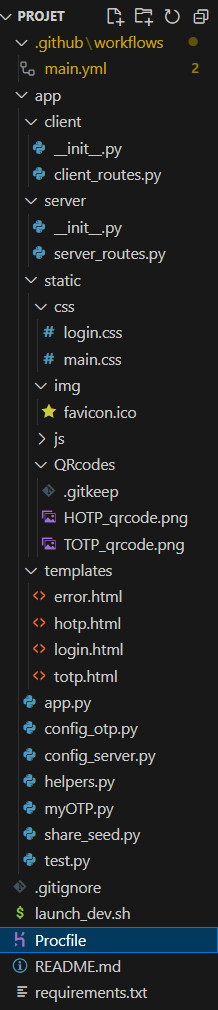
\includegraphics[scale=1]{img/C_proto/achi.png}
        \caption{architecture du projet Flask\\}
        \label{fig:proto-archi}
\end{figure}


\begin{figure}[H]
        \centering
        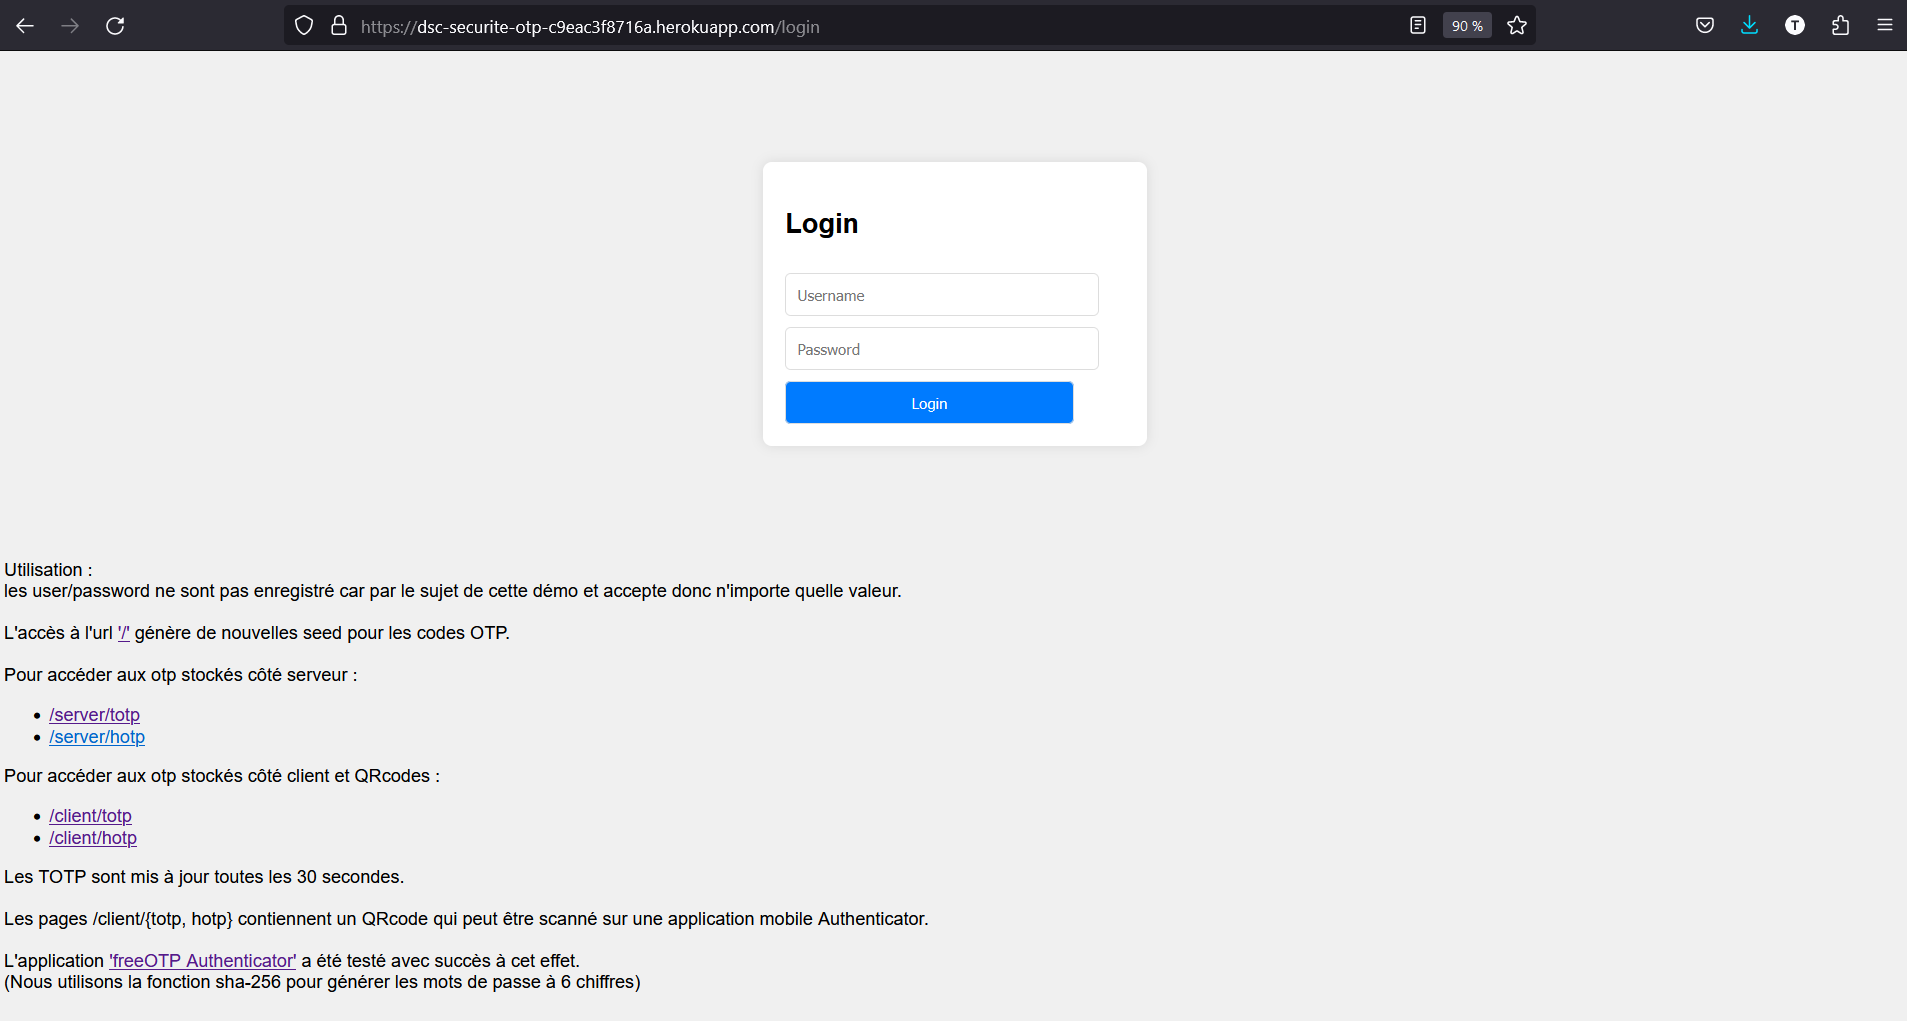
\includegraphics[scale=0.4]{img/C_proto/home.png}
        \caption{Capture d'écran de la page principale\\}
        \label{fig:home}
\end{figure}


\begin{figure}[H]
        \centering
        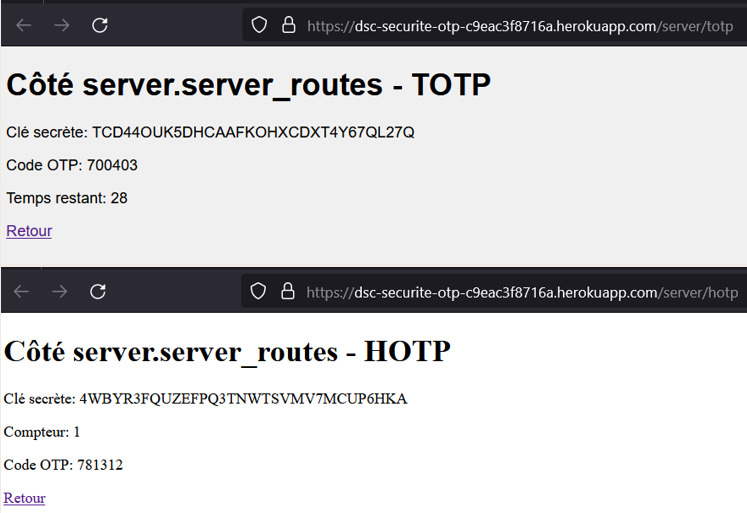
\includegraphics[scale=1]{img/C_proto/server.png}
        \caption{Pages affichant les informations du serveur\\}
        \label{fig:proto-server}
\end{figure}


\begin{figure}[H]
        \centering
        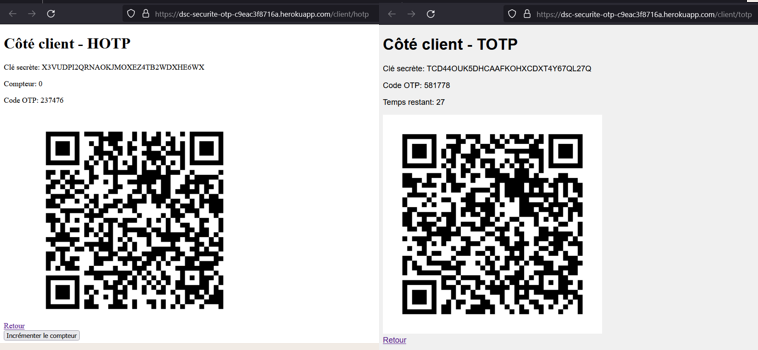
\includegraphics[scale=1]{img/C_proto/client.png}
        \caption{Pages affichant les informations du client\\}
        \label{fig:proto-client}
\end{figure}



\begin{figure}[H]
        \centering
        \includegraphics[scale=0.3]{img/C_proto/freeOTP.png\\}
        \caption{FreeOTP Authenticator}
        \label{fig:freeotp}
\end{figure}


\begin{figure}[H]
        \centering
        \includegraphics[scale=1]{img/C_proto/popup_otp.png\\}
        \caption{pop-up de saisie du code}
        \label{fig:proto-popup}
\end{figure}


\begin{figure}[H]
        \centering
        \includegraphics[scale=0.6]{img/C_proto/otp_result.png\\}
        \caption{Résultat de l'action}
        \label{fig:proto-result}
\end{figure}





\end{document}